\documentclass[preprint,12pt,authoryear]{elsarticle}
\usepackage[letterpaper,hmargin=0.9in,top=0.76in,bottom=0.78in]{geometry}
\usepackage[T1]{fontenc}
\usepackage{lmodern,textcomp}
\usepackage{booktabs,tabularx,array}
\usepackage{listings,needspace,tikz,tcolorbox,float}
\tcbuselibrary{breakable}
\definecolor{refred}{RGB}{170,43,40}
\usepackage[hidelinks]{hyperref}
\hypersetup{pdftitle={Supplementary Material: A Neuro-Symbolic Architecture for Safe and Feasible Self-Recovery in Multi-Agent Manufacturing Systems}}

\setlength{\parindent}{0pt}
\setlength{\parskip}{3pt}
\setlength{\intextsep}{6pt plus 1pt minus 1pt}
\raggedbottom
\urlstyle{tt}
\let\code\nolinkurl
\newcolumntype{Y}{>{\raggedright\arraybackslash}X}
\newtcolorbox{recordbox}[2][]{
  colback=black!2, colframe=black!40, colbacktitle=black!10,
  coltitle=black, fonttitle=\small\bfseries, title={#2},
  title after break={#2 \textnormal{(continued)}},
  arc=2pt, boxrule=0.45pt, boxsep=0pt, left=6pt, right=6pt,
  top=4pt, bottom=4pt, toptitle=4pt, bottomtitle=4pt,
  before skip=5pt, after skip=5pt, #1
}
\newcommand{\sourcepart}[1]{\par\smallskip{\small\bfseries #1\par}\nobreak\smallskip}
\lstset{
  basicstyle=\small\ttfamily,
  breaklines=true, breakatwhitespace=false, breakautoindent=false,
  columns=fullflexible, keepspaces=true, showstringspaces=false,
  upquote=true, xleftmargin=0pt, aboveskip=0pt, belowskip=0pt
}
\lstdefinestyle{recorded}{
  basicstyle=\footnotesize\ttfamily, breakindent=0pt,
  escapeinside={(*@}{@*)}
}
\newcommand{\papertitle}{A Neuro-Symbolic Architecture for Safe and Feasible Self-Recovery in Multi-Agent Manufacturing Systems}

\begin{document}
\pagestyle{plain}
\begin{center}
  {\Large\bfseries \papertitle\par}
  \medskip
  {\large Supplementary Material\par}
\end{center}

This supplement follows the decisions that connect a manufacturing failure to a recovery
program. \hyperref[sec:outline-prompt]{Appendix~A} shows how the large language model (LLM) proposed an outline and
revised it after validation. \hyperref[sec:composition-prompt]{Appendix~B} follows one accepted event into primitive
composition. \hyperref[sec:gazebo]{Appendix~C} gives the accepted events, a selected primitive sequence and
the observed Gazebo outcome for each of four runs. The worked example is Part slippage.

\appendix
\section{Recovery Outline Synthesis}
\subsection{The failure}\label{sec:failure}

During placement, \code{ur5e-4} dropped \code{gear_small} and stopped above the
assembly board. The gear came to rest on the table. The nearby arm, \code{ur5e-3},
was already holding \code{KET4_Square_4mm}. The goal was to put the loose gear in
its assigned slot and allow normal production to continue.

\begin{figure}[H]
\centering
\begin{minipage}[c]{0.51\linewidth}\centering
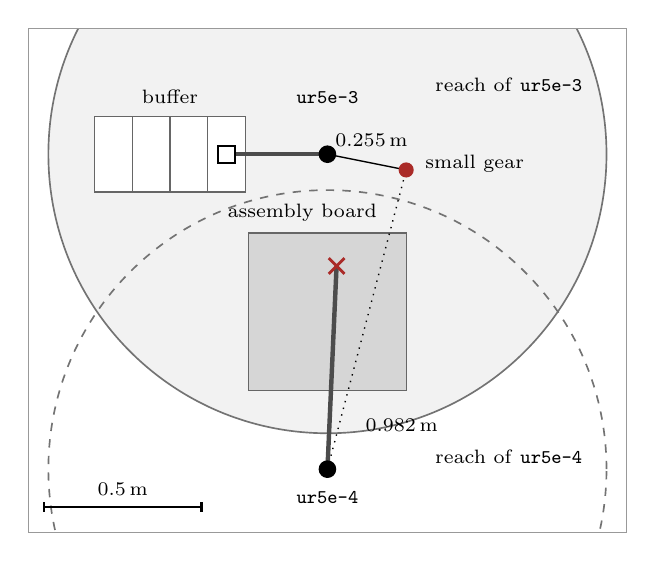
\begin{tikzpicture}[x=4.0cm,y=4.0cm,font=\scriptsize]
  \begin{scope}
    \clip (-0.95,-0.70) rectangle (0.95,0.90);
    % reach of ur5e-3 (solid, shaded) and of ur5e-4 (dashed)
    \fill[black!5] (0,0.5) circle [radius=0.886];
    \draw[black!55, line width=0.6pt] (0,0.5) circle [radius=0.886];
    \draw[black!55, line width=0.6pt, dashed] (0,-0.5) circle [radius=0.886];
    % assembly board area and the four buffer zones
    \fill[black!16] (-0.25,-0.25) rectangle (0.25,0.25);
    \draw[black!60] (-0.25,-0.25) rectangle (0.25,0.25);
    \fill[white] (-0.74,0.38) rectangle (-0.26,0.62);
    \draw[black!60] (-0.74,0.38) rectangle (-0.26,0.62);
    \draw[black!60] (-0.62,0.38) -- (-0.62,0.62) (-0.50,0.38) -- (-0.50,0.62) (-0.38,0.38) -- (-0.38,0.62);
  \end{scope}
  \draw[black!40] (-0.95,-0.70) rectangle (0.95,0.90);
  % the two distances to the gear
  \draw[black, line width=0.5pt] (0,0.5) -- (0.25,0.45);
  \draw[black, line width=0.5pt, dotted] (0,-0.5) -- (0.25,0.45);
  % arms, from base to gripper
  \draw[line width=1.6pt, black!70] (0,0.5) -- (-0.32,0.5);
  \draw[line width=1.6pt, black!70] (0,-0.5) -- (0.029,0.145);
  \fill (0,0.5) circle [radius=0.028];
  \fill (0,-0.5) circle [radius=0.028];
  % gripper of ur5e-3 with the square peg; gripper of ur5e-4 over the gear's slot
  \filldraw[fill=white, draw=black, line width=0.6pt] (-0.347,0.473) rectangle (-0.293,0.527);
  \draw[refred, line width=1pt] (0.004,0.120) -- (0.054,0.170) (0.004,0.170) -- (0.054,0.120);
  % the fallen gear
  \fill[refred] (0.25,0.45) circle [radius=0.024];
  % labels
  \node[anchor=south] at (0,0.63) {\texttt{ur5e-3}};
  \node[anchor=north] at (0,-0.54) {\texttt{ur5e-4}};
  \node[anchor=south] at (-0.50,0.63) {buffer};
  \node[anchor=south] at (-0.08,0.255) {assembly board};
  \node[anchor=west] at (0.28,0.47) {small gear};
  \node[anchor=south] at (0.14,0.495) {0.255\,m};
  \node[anchor=west] at (0.09,-0.36) {0.982\,m};
  \node[anchor=east] at (0.84,0.72) {reach of \texttt{ur5e-3}};
  \node[anchor=east] at (0.84,-0.46) {reach of \texttt{ur5e-4}};
  % scale bar
  \draw[line width=0.8pt] (-0.90,-0.62) -- (-0.40,-0.62);
  \draw[line width=0.8pt] (-0.90,-0.635) -- (-0.90,-0.605) (-0.40,-0.635) -- (-0.40,-0.605);
  \node[anchor=south] at (-0.65,-0.615) {0.5\,m};
\end{tikzpicture}
\end{minipage}\hfill
\begin{minipage}[c]{0.46\linewidth}
\small\raggedright
The dot marks \code{gear_small}. The solid and dashed arcs show the
horizontal reach of \code{ur5e-3} and \code{ur5e-4}, respectively
(0.886\,m for each arm).
\par\smallskip
The square marks the gripper of \code{ur5e-3}, holding \code{KET4_Square_4mm}
at the buffer. The cross marks the stopped gripper of \code{ur5e-4} inside
the assembly board area.
\end{minipage}
\caption{Part slippage seen from above. The authors reconstructed the scene from the recorded positions. The initial prompt supplied the gear position. The requested distances from the gear to the robot bases appeared on turn~2.}
\label{fig:failure-scene}
\end{figure}

The initial prompt gave the gear's measured position. On turn~1 the LLM requested
eight facts, including \code{/parts/gear_small/pose_relations}. The turn~2 prompt
placed the gear 0.255\,m from the base of \code{ur5e-3} and 0.982\,m from the
base of \code{ur5e-4}. Of those two arms, only \code{ur5e-3} could reach it.
The LLM therefore needed a way to free that arm's gripper.

\clearpage
\subsection{What the LLM receives}\label{sec:outline-prompt}
Table~\ref{tab:outline-blocks} describes the initial event-level Framework prompt.
The worked run used Claude Opus~5.5 at medium reasoning effort.

\begin{table}[H]\centering\small
\caption{What the first outline prompt supplies.}\label{tab:outline-blocks}
\begin{tabularx}{\linewidth}{@{}>{\raggedright\arraybackslash}p{.30\linewidth}Y@{}}
\toprule
Prompt block & Purpose \\
\midrule
Task and Role, Failure, Recovery Goal & Define the next decision, the measured starting state and the target slot. \\
Candidate Rules & Require the acting resource and the state changes that its event would establish. These are the values the agents check. \\
Knowledge Base & Lists eleven reference paths for requesting facts before proposing an event. \\
Resources and Parts & Give the states of 12 resources and 12 parts, including the actions available to each resource, before the first lookup. \\
\bottomrule
\end{tabularx}
\end{table}

The turn~1 user message lists the failure, goal and available evidence before any lookup. The selections below keep the measurements, one lookup path, one robot and one part involved in choosing an arm. The full inventories, other lookup paths and rules for unrelated actions are omitted. Bold labels identify the source blocks. The system message supplies the reply schema. The final instruction comes from the separate outline-level prompt.

\begin{recordbox}[breakable]{Outline prompts \enspace Part slippage}
\sourcepart{Turn 1 prompt \enspace Task and Role}
\begin{lstlisting}[style=recorded]
Plan how to get from the current state to the Recovery Goal. Propose 2(*@{\rmfamily\textendash}@*)5 different ways to do the next step of that plan, most preferred first. The first one in your order that passes every check becomes the next recovery event; the others are dropped.
\end{lstlisting}
\sourcepart{Turn 1 prompt \enspace Failure}
\begin{lstlisting}[style=recorded]
- gear_small: not held, not at any station, measured at (0.250, 0.450, 1.025)
- ur5e-4: measured pose (0.029, 0.145, 1.289), inside assembly_board-v1
\end{lstlisting}
\sourcepart{Turn 1 prompt \enspace Recovery Goal}
\begin{lstlisting}[style=recorded]
- gear_small: part_location assembly_board-v1 (target Gear_Plate/Gear_Shaft_1) (normally ur5e-4's place_insert; ur5e-4 failed)
\end{lstlisting}
\sourcepart{Turn 1 prompt \enspace Candidate Rules}
\begin{lstlisting}[style=recorded]
- One event per candidate, by one resource: `outline_id`, `event_name` (what it achieves; new names allowed), `resource`, `part_name` (if a part is involved), `expected_end_state`, `neighbor_end_state` (if needed), `rationale` (the fact it relies on).
Give `pose` only for a position nothing else gives: an arm's pick or place target comes from the part or the place when it declares compute_pick_targets or compute_place_targets, a named pose gives its own position, and a mobile base's reachable location gives its pose.
\end{lstlisting}
\sourcepart{Turn 1 prompt \enspace Knowledge Base}
\begin{lstlisting}[style=recorded]
- /parts/<name>/pose_relations: which areas contain its measured position (one point, not its full extent), which declared places contain it, and how far it lies from each resource's workspace bounds
\end{lstlisting}
\tcbbreak
\sourcepart{Turn 1 prompt \enspace Resources}
\begin{lstlisting}[style=recorded]
ur5e-3 (robot)  picked; held_part KET4_Square_4mm; resource_location Buffer For Machined parts; pose (-0.320, 0.500, 1.501); capabilities: reachable locations Buffer For Machined parts, assembly_board-v1, Exit; workspace bounds; actions: compute_pick_targets; compute_place_targets
\end{lstlisting}
\sourcepart{Turn 1 prompt \enspace Parts}
\begin{lstlisting}[style=recorded]
gear_small  not held, not at any station, measured at (0.250, 0.450, 1.025), assembly target Gear_Plate/Gear_Shaft_1; processes: print_part completed
\end{lstlisting}
\sourcepart{Turn 1 system prompt \enspace Required event fields}
\begin{lstlisting}[style=recorded]
"required": ["outline_id", "event_name", "resource", "expected_end_state", "rationale"]
\end{lstlisting}
\sourcepart{Outline-level comparison prompt \enspace Task and Role}
\begin{lstlisting}[style=recorded]
Give the whole plan in `events`: every recovery event, in the order they happen.
\end{lstlisting}
\end{recordbox}

At the event level, the Framework checks candidates in the LLM's order.
Baseline and Informed baseline take the first candidate. Informed baseline
also supplies the seven safety rules. At the outline level each method asks for
the complete sequence in a single reply.

\Needspace{21\baselineskip}
\subsection{The run, turn by turn}\label{sec:turns}
The Resource Agent (RA) checks feasibility. The Central Controller Agent (CCA)
checks the safety of feasible candidates. The first candidate that passes both
checks becomes the next event in the projected outline.

\begin{table}[H]\centering\small
\caption{Seven outline turns in the Part slippage run.}\label{tab:turns}
\begin{tabularx}{\linewidth}{@{}r Y Y@{}}
\toprule
Turn & LLM decision & Check or result \\
\midrule
1 & Request eight facts, including the gear's position relative to the arms. & The requested values appear on turn~2. \\
2 & Place the held peg on the board or stage it in the buffer. & The CCA refuses the board placement. Staging passes and becomes event~1. \\
3 & Retract \code{ur5e-4} to its home pose. & Event~2 passes, clearing the board in the projected state. \\
4 & Pick the gear with \code{ur5e-3}. Both candidates specify an arm pose. & The RA refuses both candidates. \\
5 & Revise the pick while retaining \code{gear_small} as the intended held part. & Event~3 passes. \\
6 & Place the gear in its board slot. & Event~4 passes. \\
7 & Declare \code{recovery_complete}. & The CCA returns \code{NONBLOCKING} for continuation of normal production. \\
\bottomrule
\end{tabularx}
\end{table}

\subsection{How feedback changed the outline}
On turn~2, the CCA
found that the proposed board placement would put both arms in the protected
area, violating \code{SAFE_shared_area_mutex}. The next candidate staged the peg in the buffer and passed both checks. The turn~3 prompt reported both outcomes, and the LLM then
proposed retracting \code{ur5e-4}.

On turn~4, neither pick candidate passed. The RA found that the gear's recorded
position already supplied the pick target. Turn~5 kept the event name
\code{pick_dropped_gear_small_ur5e3} and removed the proposed robot pose.

\Needspace{16\baselineskip}
\begin{recordbox}[breakable]{Outline validation \enspace From the first lookup to the accepted pick}
\sourcepart{Turn 1 LLM reply \enspace Decision and first of eight requested paths}
\begin{lstlisting}[style=recorded]
"decision": "need_context",
"context_requests": ["/parts/gear_small/pose_relations",
\end{lstlisting}
\sourcepart{Turn 2 prompt \enspace Retrieved context}
\begin{lstlisting}[style=recorded]
"reachability": ["Buffer For Machined parts", "assembly_board-v1", "Exit"]
\end{lstlisting}
\sourcepart{Turn 2 prompt \enspace Retrieved current values}
\begin{lstlisting}[style=recorded]
"ur5e-3": {"max_xy_radius_m": 0.886, "tolerance_m": 0.01, "xy_distance_m": 0.255, "z_m": 1.025, "z_range_m": [0.971, 1.121]}
\end{lstlisting}
\sourcepart{Turn 3 prompt \enspace Recovery Events So Far (planned, not executed)}
\begin{lstlisting}[style=recorded]
"outline_id": "RECOVERY_SEQ1",
"event_name": "stage_KET4_in_buffer",
\end{lstlisting}
\sourcepart{Turn 3 prompt \enspace Validation Feedback}
\begin{lstlisting}[style=recorded]
SAFE_shared_area_mutex (At most one resource may occupy the assembly_board-v1 destination area at any time.) is broken during the event: ur5e-3 is in assembly_board-v1 while ur5e-4 is in assembly_board-v1
\end{lstlisting}
\par\medskip\hrule\smallskip
\begin{minipage}[t]{0.483\linewidth}
{\small\bfseries LLM reply \enspace Turn 4, proposed}\par\smallskip
\begin{lstlisting}[style=recorded]
"expected_end_state": {
  "held_part": "gear_small",
  "resource_state": "picked",
  "resource_location": null,
  "pose": {"x": 0.25, "y": 0.45,
           "z": 1.243},
  "part_location": "ur5e-3"
}
\end{lstlisting}
\end{minipage}\hfill
\begin{minipage}[t]{0.483\linewidth}
{\small\bfseries LLM reply \enspace Turn 5, accepted}\par\smallskip
\begin{lstlisting}[style=recorded]
"expected_end_state": {
  "resource_state": "picked",
  "held_part": "gear_small",
  "resource_location": null,
  "part_location": "ur5e-3"
}
\end{lstlisting}
\end{minipage}
\par\medskip\hrule\smallskip
{\small\bfseries Prompt \enspace Turn 5, RA finding on the first candidate}\par\smallskip
\begin{lstlisting}[style=recorded]
gear_small's recorded position gives ur5e-3's target, so this event takes no pose; it states {x: 0.250, y: 0.450, z: 1.243}
\end{lstlisting}
\sourcepart{Turn 6 prompt \enspace Missing context}
\begin{lstlisting}[style=recorded]
"ref": "/parts/gear_small/pose_relations",
"error": "NEEDS_CONTEXT: /parts/gear_small/observed_pose requires a new observation after the projected part transition"
\end{lstlisting}
\end{recordbox}

The turn~2 entries show the reach of \code{ur5e-3} and its measured distance to the gear. The turn~3 entries identify the accepted staging event and explain the refusal of the earlier candidate. After the pick, the old gear observation could no longer supply its pose relative to the arms. Repeated inventories, the other lookup responses and the second refusal of the same pose rule are omitted here. Turn~7 closed the outline with \code{recovery_complete}. The CCA found the resulting state \code{NONBLOCKING} for normal production. The four accepted events appear in \hyperref[sec:gazebo-slippage]{Appendix~C.1}.

\clearpage
\section{Primitive Composition of Event 3}
\setcounter{table}{0}
\renewcommand*{\theHtable}{B.\arabic{table}}
\subsection{The accepted event becomes the prompt}\label{sec:composition-prompt}

The outline fixed the acting resource, the gear and the intended end state.
On call~5 the RA gave the LLM this accepted event and asked it to compose the
pick from the primitives of \code{ur5e-3}. Calls~5--7 address this event.

\begin{table}[H]\centering\small
\caption{What the composition prompt supplies on call~5.}
\begin{tabularx}{\linewidth}{@{}>{\raggedright\arraybackslash}p{.32\linewidth}Y@{}}
\toprule
Prompt block & Purpose \\
\midrule
Task and Role, Visible Primitive Catalog & Limit the program to the active event and identify the eight primitives available to its resource. \\
Published Ref Schema, Available Capability Decompositions & Give 15 lookup paths and five nominal function names. The LLM can request a primitive contract or an example of how the robot performs a nominal task. \\
Active DES Transition, Transition Authoring Cursor, Accepted Outline Summary & Identify the active event, its place in this composition request and the state its program must establish. \\
Named Pose Rules & Limit named movements to the poses advertised by this resource. \\
Output Contract, RA composition validation & Require values in numeric parameters to come from explicit references. The RA checks the ordered steps against the event's intended end state. \\
\bottomrule
\end{tabularx}
\end{table}

The prompt supplies the accepted event inline. The entries below show how the LLM identifies its robot, locates a contract and learns which values its program must establish. We show one catalog entry, one lookup path and two nominal functions used in this pick. The other entries, repeated event description, rules for other resources and remaining schema fields are omitted. JSON spacing is condensed for print.

\begin{recordbox}[breakable]{Primitive composition prompt \enspace Call 5, event 3}
\sourcepart{Task and Role}
\begin{lstlisting}[style=recorded]
Author primitive_steps for ONLY the active DES transition, using only the visible primitive catalog for the active resource.
\end{lstlisting}
\sourcepart{Visible Primitive Catalog}
\begin{lstlisting}[style=recorded]
{"name": "compute_pick_targets"}
\end{lstlisting}
\sourcepart{Published Ref Schema (for context\_requests)}
\begin{lstlisting}[style=recorded]
{"ref": "/primitive_contracts/<name>", "description": "contract card for one visible primitive"}
\end{lstlisting}
\sourcepart{Available Capability Decompositions}
\begin{lstlisting}[style=recorded]
"pick_approach", "pick_grasp"
\end{lstlisting}
\sourcepart{Active DES Transition (token)}
\begin{lstlisting}[style=recorded]
"outline_id": "RECOVERY_SEQ3",
"resource_jid": "recovery-resource-3@localhost",
"action": "pick_dropped_gear_small_ur5e3"
\end{lstlisting}
\tcbbreak
\sourcepart{Active DES Transition (full event)}
\begin{lstlisting}[style=recorded]
"event_name": "pick_dropped_gear_small_ur5e3",
"part_name": "gear_small",
"expected_start_state": {"held_part": null, "part_location": null, "resource_location": "Buffer For Machined parts", "resource_state": "placed"},
"expected_end_state": {"resource_state": "picked", "held_part": "gear_small", "resource_location": null, "part_location": "recovery-resource-3@localhost"}
\end{lstlisting}
\sourcepart{Transition Authoring Cursor}
\begin{lstlisting}[style=recorded]
{"active_index": 0, "accepted_outline_count": 1, "remaining_events_count": 1}
\end{lstlisting}
\sourcepart{Accepted Outline Summary (context for active event)}
\begin{lstlisting}[style=recorded]
- RECOVERY_SEQ3 / recovery-resource-3@localhost / gear_small -> pick_dropped_gear_small_ur5e3 to recovery-resource-3@localhost
\end{lstlisting}
\sourcepart{Named Pose Rules}
\begin{lstlisting}[style=recorded]
["home"]
- move_to_named_pose may only use named poses advertised for the active resource.
\end{lstlisting}
\sourcepart{Output Contract}
\begin{lstlisting}[style=recorded]
- Each step MUST include params. Every number in params is a {"context_ref": ...}; strings and booleans may be literals from served context.
\end{lstlisting}
\sourcepart{RA composition validation}
\begin{lstlisting}[style=recorded]
RA composition validation: author an ordered program that establishes every intended resource and part postcondition from declared effects or what the checks find.
\end{lstlisting}
\sourcepart{System prompt \enspace Reply decisions}
\begin{lstlisting}[style=recorded]
"enum": ["primitive_steps_ready", "need_context", "need_primitive_revision"]
\end{lstlisting}
\end{recordbox}

\subsection{The revision and accepted program}\label{sec:pick-program}
On call~5 the LLM requested the primitive contracts, the robot's nominal pick
steps, its projected state and model, and the gear observation. The call~6 prompt below shows the model identifier and the retrieved pick contract. The remaining model and contract fields are omitted because the revision concerns the source of the pick target. On call~6 the LLM
bound the gear's observed coordinates directly to \code{compute_pick_targets}
and supplied a source for them. The RA flagged these inputs. On call~7 the
revised calculation took only the part name and read the recorded pose itself.

\begin{recordbox}[breakable]{Primitive composition revision \enspace Calls 5--7, event 3}
\sourcepart{Call 5 LLM reply \enspace Decision and first requested contract}
\begin{lstlisting}[style=recorded]
"decision": "need_context",
"context_requests": ["/primitive_contracts/compute_pick_targets",
\end{lstlisting}
\sourcepart{Call 6 prompt \enspace Served Context: resource model}
\begin{lstlisting}[style=recorded]
"/resources/recovery-resource-3@localhost/recovery_des_model": {
  "model_type": "extended_finite_automaton",
  "resource_jid": "recovery-resource-3@localhost",
\end{lstlisting}
\sourcepart{Call 6 prompt \enspace Served Context (retrieved earlier in this event)}
\begin{lstlisting}[style=recorded]
"name": "compute_pick_targets",
"description": "Compute vertical pick target positions from world object geometry and configured end-effector/TCP feedback without moving. The frames must agree."
\end{lstlisting}
\tcbbreak
{\small\bfseries LLM reply \enspace Call 6, proposed first step}\par\smallskip
\begin{lstlisting}[style=recorded]
{"primitive": "compute_pick_targets", "params": {
  "part_name": "gear_small",
  "target_pose": {
    "x": {"context_ref": "/parts/gear_small/observed_pose/x"},
    "y": {"context_ref": "/parts/gear_small/observed_pose/y"},
    "z": {"context_ref": "/parts/gear_small/observed_pose/z"},
    "model_name": {"context_ref": "/parts/gear_small/target/model_name"}
  },
  "target_pose_source": "observed_pose"}}
\end{lstlisting}
\par\medskip
{\small\bfseries Prompt \enspace Call 7, Previous Validation Feedback (read first)}\par\smallskip
\begin{lstlisting}
compute_pick_targets: target_pose {'x': 0.24992089458069847, 'y': 0.44999843654915983, 'z': 1.0249998633209128, 'model_name': 'gear_small'} differs from None, the input the composition's calculation reads; compute_pick_targets: target_pose_source 'observed_pose' differs from '', the input the composition's calculation reads
\end{lstlisting}
\par\medskip
{\small\bfseries LLM reply \enspace Call 7, accepted first step}\par\smallskip
\begin{lstlisting}
{"primitive": "compute_pick_targets", "params": {"part_name": "gear_small"}},
\end{lstlisting}
\par\smallskip
\sourcepart{LLM reply \enspace Call 7, step 2 uses the output of step 1}
\begin{lstlisting}[style=recorded]
"x": {"context_ref": "event_facts.pick_targets.gear_small.approach_pose.x"},
\end{lstlisting}
\end{recordbox}

\begin{table}[H]
\centering\small
\caption{Accepted program for event~3, \code{pick_dropped_gear_small_ur5e3}. Cartesian positions $(x,y,z)$ are in metres, rounded to three decimal places.}\label{tab:pick}
\begin{tabularx}{\linewidth}{@{}r l Y Y@{}}
\toprule
Step & Primitive & Written by the LLM & Resolved by the RA \\
\midrule
1 & \code{compute_pick_targets} & Part name \code{gear_small}. & Approach, target and retreat poses from the recorded gear position. \\
2 & \code{move_cartesian} & References to \code{approach_pose}. & $(0.250,\,0.450,\,1.303)$ above the gear. \\
3 & \code{move_cartesian} & References to \code{target_pose}. & $(0.250,\,0.450,\,1.253)$ at the pick target. \\
4 & \code{grasp_part} & Part name and a reference to its model name. & Both names resolve to \code{gear_small}. \\
5 & \code{move_cartesian} & References to \code{retreat_pose}. & $(0.250,\,0.450,\,1.303)$ with the gear held. \\
\bottomrule
\end{tabularx}
\end{table}

The RA resolved the references during composition validation. Step~1 produced
the approach, target and retreat poses. Steps~2, 3 and~5 used them in that
order. The five-step program established the end state of event~3.

\clearpage
\section{Recovery Runs Executed in Gazebo}\label{sec:gazebo}
\setcounter{table}{0}
\renewcommand*{\theHtable}{C.\arabic{table}}

For each scenario, we compared the passing event-level Framework outlines from
all three models and selected one with the fewest events.
For each run, the table reports how many LLM calls were needed to compose
the accepted events, how many primitive steps those programs contained, and
how many events completed in Gazebo. The 29 accepted events contained 121
primitive steps in total. Each case gives the complete outline, then expands the numbered event shown in bold into its accepted primitive steps. The final paragraph reports what happened during the Gazebo replay.

\begin{center}
\small
\setlength{\tabcolsep}{4pt}
\begin{tabularx}{\linewidth}{@{}Y l c c c c@{}}
\toprule
Scenario & Model & \shortstack{Outline\\turns} & \shortstack{Composition\\calls} & \shortstack{Accepted\\primitive steps} & \shortstack{Events\\completed} \\
\midrule
Part slippage & Claude Opus 5.5 & 7 & 9 & 16 & 4 of 4 \\
Conveyor breakdown & Claude Opus 5.5 & 12 & 15 & 23 & 7 of 7 \\
ur5e-1 breakdown & GPT-6.1 Sol & 11 & 19 & 20 & 4 of 4 \\
Machining breakdown during part processing & GPT-6.1 Sol & 20 & 49 & 62 & 14 of 14 \\
\bottomrule
\end{tabularx}
\end{center}

\subsection{Part slippage}\label{sec:gazebo-slippage}
The gear fell while \code{ur5e-4} was placing it. The arm that could reach it, \code{ur5e-3}, was holding the square peg.

{\small
\begin{tabularx}{\linewidth}{@{}r Y l Y@{}}
\toprule
Event & Accepted event name & Resource & Intended change \\
\midrule
1 & \code{stage_KET4_in_buffer} & \code{ur5e-3} & Free the gripper and leave the square peg in buffer zone 1. \\
2 & \code{retract_ur5e4_home_clear_board} & \code{ur5e-4} & Leave the arm idle at its home pose. \\
3 & \code{pick_dropped_gear_small_ur5e3} & \code{ur5e-3} & Hold the loose gear in the gripper. \\
\textbf{4} & \code{place_gear_small_on_board_ur5e3} & \code{ur5e-3} & Leave the gear on the board and record assembly at its assigned slot. \\
\bottomrule
\end{tabularx}\par}

\Needspace{8\baselineskip}
\textbf{Primitive program for event~4} \enspace \code{place_gear_small_on_board_ur5e3}\par
Event~3 ends with the gear in the gripper (\hyperref[tab:pick]{Table~\ref*{tab:pick}}). Event~4 must release it at \code{Gear_Plate/Gear_Shaft_1}.

{\small
\begin{tabularx}{\linewidth}{@{}r l Y@{}}
\toprule
Step & Primitive & Operation \\
\midrule
1 & \code{compute_place_targets} & Calculate the placement poses and slot coordinates for the gear on the assembly board. \\
2 & \code{move_cartesian} & Move above the assigned slot at the approach pose. \\
3 & \code{move_cartesian} & Descend to the placement target. \\
4 & \code{release_part} & Release the gear using the calculated assembly slot. \\
5 & \code{move_cartesian} & Withdraw to the retreat pose above the board. \\
\bottomrule
\end{tabularx}\par}
At step~4, \code{assembly_slot.slot_x} reads \code{event_facts.place_targets.gear_small.slot_x}, which step~1 calculated for this gear.

\smallskip
\textbf{Gazebo outcome.} The staging calculation in event~1 could not resolve the buffer geometry live. The staging motion used the saved parameters. After \code{ur5e-4} retracted, Gazebo recorded \code{gear_small} attached to \code{ur5e-3} after event~3 and released after event~4. The gear's final position on the board was $(0.029,\,0.145,\,1.039)$\,m.

\clearpage
\subsection{Conveyor breakdown}
The Conveyor became unavailable while \code{ur5e-1} held the machined square peg, \code{KET4_Square_4mm}. The M1 staging tray gave the fixed arm and KMR a common handoff point.

{\small
\begin{tabularx}{\linewidth}{@{}r Y l Y@{}}
\toprule
Event & Accepted event name & Resource & Intended change \\
\midrule
1 & \code{place_on_M1_staging_tray} & \code{ur5e-1} & Leave the peg on the M1 staging tray and empty the gripper. \\
2 & \code{navigate_KMR_to_M1} & \code{KMR} & Bring the mobile base to M1. \\
3 & \code{ur5e1_retract_home} & \code{ur5e-1} & Leave the fixed arm idle at home. \\
\textbf{4} & \code{kmr_pick_from_M1_staging_tray} & \code{KMR} & Leave KMR carrying the peg and the M1 staging tray empty. \\
5 & \code{kmr_move_base_to_buffer} & \code{KMR} & Move the loaded base to its proposed pose beside the buffer. \\
6 & \code{kmr_place_on_buffer_zone_1} & \code{KMR} & Leave the peg in buffer zone 1 and empty the gripper. \\
7 & \code{kmr_stow_arm_and_return_to_storage} & \code{KMR} & Return KMR to Storage in the idle state. \\
\bottomrule
\end{tabularx}\par}

\Needspace{8\baselineskip}
\textbf{Primitive program for event~4} \enspace \code{kmr_pick_from_M1_staging_tray}\par
By event~4 the base is at M1 and the fixed arm has withdrawn. The program therefore begins at the tray.

{\small
\begin{tabularx}{\linewidth}{@{}r l Y@{}}
\toprule
Step & Primitive & Operation \\
\midrule
1 & \code{detect_parts} & Detect the staged peg from the M1 dock. \\
2 & \code{compute_pick_targets} & Calculate the approach, grasp and lift targets. \\
3 & \code{move_to_named_pose} & Move the KMR arm to its named transport pose. \\
4 & \code{move_cartesian} & Move to the tray approach using the calculated seed. \\
5 & \code{move_cartesian} & Move the gripper to the pick target. \\
6 & \code{grasp_part} & Grasp the square peg. \\
7 & \code{move_cartesian} & Lift the peg clear of the tray along the calculated lift waypoints. \\
\bottomrule
\end{tabularx}\par}
Step~4 reads \code{target} from \code{/event_facts/pick_targets/KET4_Square_4mm/approach}.

\smallskip
\textbf{Gazebo outcome.} After event~4, Gazebo recorded KMR at M1 holding \code{KET4_Square_4mm}. KMR released the peg in buffer zone~1. Its final observation placed the empty mobile robot back at Storage.

\clearpage
\subsection{ur5e-1 breakdown}
The gripper on \code{ur5e-1} failed before the arm could transfer the completed square peg from M1 to the Conveyor. KMR took over the transfer.

{\small
\begin{tabularx}{\linewidth}{@{}r Y l Y@{}}
\toprule
Event & Accepted event name & Resource & Intended change \\
\midrule
1 & Retract the empty arm to its named home pose & \code{ur5e-1} & Leave the empty arm idle at home. \\
2 & Retrieve the completed part from M1 with KMR & \code{KMR} & Hold the square peg on KMR and leave M1 empty. \\
\textbf{3} & Deliver to conveyor loading position 1 using a south-facing base heading & \code{KMR} & Leave the peg at loading position 1 and the empty KMR base facing south. \\
4 & Return KMR to Storage and verify idle readiness & \code{KMR} & Leave KMR empty and idle at Storage. \\
\bottomrule
\end{tabularx}\par}

\Needspace{8\baselineskip}
\textbf{Primitive program for event~3} \enspace Deliver to conveyor loading position 1 using a south-facing base heading\par
Event~2 ends with KMR holding the peg at M1. Event~3 specifies both the loading position and the base heading from which KMR can reach it.

{\small
\begin{tabularx}{\linewidth}{@{}r l Y@{}}
\toprule
Step & Primitive & Operation \\
\midrule
1 & \code{move_to_named_pose} & Stow the loaded arm in the transport pose. \\
2 & \code{move_base} & Drive to the base pose specified in the event, facing south. \\
3 & \code{compute_place_targets} & Calculate placement targets from the part pose and recorded grasp transform. \\
4 & \code{move_cartesian} & Follow the transfer waypoints to the approach pose. \\
5 & \code{move_cartesian} & Move to the placement target at loading position 1. \\
6 & \code{release_part} & Release the peg using the same grasp transform as in step 3. \\
7 & \code{move_cartesian} & Lift the gripper to the retreat pose. \\
8 & \code{move_cartesian} & Follow the withdrawal waypoints back to the transport configuration. \\
\bottomrule
\end{tabularx}\par}
The yaw component of \code{move_base}'s \code{target_pose} in step~2 reads \code{/outline_event/expected_end_state/pose/yaw}. The accepted value was $-\pi/2$ radians.

\smallskip
\textbf{Gazebo outcome.} At release, Gazebo measured the peg at $(-4.050,\,0.501,\,1.015)$\,m at loading position~1 and reported an empty gripper. KMR then returned to Storage.

\clearpage
\subsection{Machining breakdown during part processing}
M1 failed during the square trim of \code{KET4_Square_4mm}. M2 could perform that operation, but it was already trimming the round peg, \code{RGOCG4-50_Round_4mm}.

{\footnotesize
\setlength{\tabcolsep}{3pt}
\begin{tabularx}{\linewidth}{@{}r >{\raggedright\arraybackslash}p{.43\linewidth} l Y@{}}
\toprule
Event & Accepted event name & Resource & Intended change \\
\midrule
1 & Pause M2's round-part job for temporary unloading & \code{M2} & Pause the active circle trim on M2. \\
\textbf{2} & Unload the paused round part into M2's staging tray & \code{ur5e-2} & Leave M2 idle and the round peg on its staging tray. \\
3 & Navigate to M1 and retrieve the interrupted square part & \code{KMR} & Take custody of the interrupted square peg at M1. \\
4 & Select M2's square program before loading & \code{M2} & Set the selected program to square. \\
5 & Return ur5e-2 home to clear M2 access & \code{ur5e-2} & Leave the arm idle at home. \\
6 & Navigate to M2 and load the interrupted square part & \code{KMR} & Leave the square peg loaded in M2. \\
7 & Navigate KMR to Storage to clear M2 & \code{KMR} & Move the mobile base back to Storage. \\
8 & Start the square-part job on M2 & \code{M2} & Set the square trim running on M2. \\
9 & Await and verify completion of square trimming on M2 & \code{M2} & Record the completed square trim and clear the current process. \\
10 & Transfer the completed square part from M2 to Conveyor & \code{ur5e-2} & Leave the square peg at Conveyor loading position 2 and M2 idle. \\
11 & Reload the paused round part from M2's staging tray & \code{ur5e-2} & Load the round peg back into M2 and clear its staging tray. \\
12 & Return ur5e-2 home to clear M2 for resumed processing & \code{ur5e-2} & Leave the arm idle at home. \\
13 & Restore M2's circle program before a separate resume event & \code{M2} & Set the selected program to circle. \\
14 & Resume the reloaded paused round-part job & \code{M2} & Resume the circle trim on M2. \\
\bottomrule
\end{tabularx}\par}

\Needspace{8\baselineskip}
\textbf{Primitive program for event~2} \enspace Unload the paused round part into M2's staging tray\par
Event~2 frees M2 for the square peg while keeping the round peg available to reload at event~11. Steps~1--6 remove it from M2, and steps~7--11 place it on the tray.

{\small
\begin{tabularx}{\linewidth}{@{}r l Y@{}}
\toprule
Step & Primitive & Operation \\
\midrule
1 & \code{detect_parts} & Detect the round peg in M2. \\
2 & \code{compute_pick_targets} & Calculate pick targets for the round peg. \\
3 & \code{move_cartesian} & Approach the round peg in M2. \\
4 & \code{move_cartesian} & Descend to the pick target inside M2. \\
5 & \code{grasp_part} & Grasp the round peg. \\
6 & \code{move_cartesian} & Withdraw with the peg to the pick retreat pose. \\
7 & \code{compute_place_targets} & Calculate placement poses for the M2 staging tray. \\
8 & \code{move_cartesian} & Move to the placement approach above the tray. \\
9 & \code{move_cartesian} & Descend to the placement target on the tray. \\
10 & \code{release_part} & Release the round peg. \\
11 & \code{move_cartesian} & Withdraw the empty gripper to the placement retreat pose. \\
\bottomrule
\end{tabularx}\par}
For \texttt{M2 staging tray} (step~7), step~8 binds $x$ to \code{/event_facts/place_targets/RGOCG4-50_Round_4mm/approach_pose/x}.

\smallskip
\textbf{Gazebo outcome.} The round peg rested on the M2 staging tray while M2 finished the square trim. After \code{ur5e-2} transferred the square peg to the Conveyor and reloaded the round peg, M2 accepted \code{resume_job} for the original job, \code{environment_24}.

\end{document}
